\documentclass{beamer}
\usepackage[utf8]{inputenc}
\usepackage[T1]{fontenc}
\usepackage{lmodern}
\usepackage{graphicx}
\usepackage{amsmath, amssymb, graphicx}
\usepackage{listings}
\usepackage{color}
\usepackage{subcaption}

%\usepackage{beamerthemeshadow}
%\beamersetuncovermixins{\opaqueness<1>{25}}{\opaqueness<2->{15}}
\usetheme{Ilmenau}
\begin{document}
\title{Free Surface Flows} 
\date{03.02.2014}
\author{M. Farahani, E. Wolter, A. Hahn}
\frame{\titlepage}
%\frame{\frametitle{Structure}\tableofcontents} 

\section{Free Surface Flow} 
\subsection{Application}

\begin{frame}
 		\begin{figure}
 			\begin{subfigure}[c]{0.3\textwidth}
 		 	      \includegraphics[width=1\textwidth]{pic/images.jpg}
 		 	\end{subfigure} 		 	
 		 	 \begin{subfigure}[c]{0.3\textwidth}
 		 	      \includegraphics[width=1\textwidth]{pic/images1.jpg}
 		 	\end{subfigure}
 		 	
 		 	\vspace{1em}
 		 	
 			\begin{subfigure}[c]{0.3\textwidth}
 		 	      \includegraphics[width=1\textwidth]{pic/images2.jpg}
 		 	\end{subfigure}
 		 	 \begin{subfigure}[c]{0.3\textwidth}
 		 	      \includegraphics[width=1\textwidth]{pic/images3.jpg}
 		 	\end{subfigure}   
 		\end{figure}
\end{frame}	

\subsection{Theory}
 \begin{frame}{Theory}
   \begin{columns}
	 	\begin{column}[c]{0.35\textwidth}
			\begin{figure}
				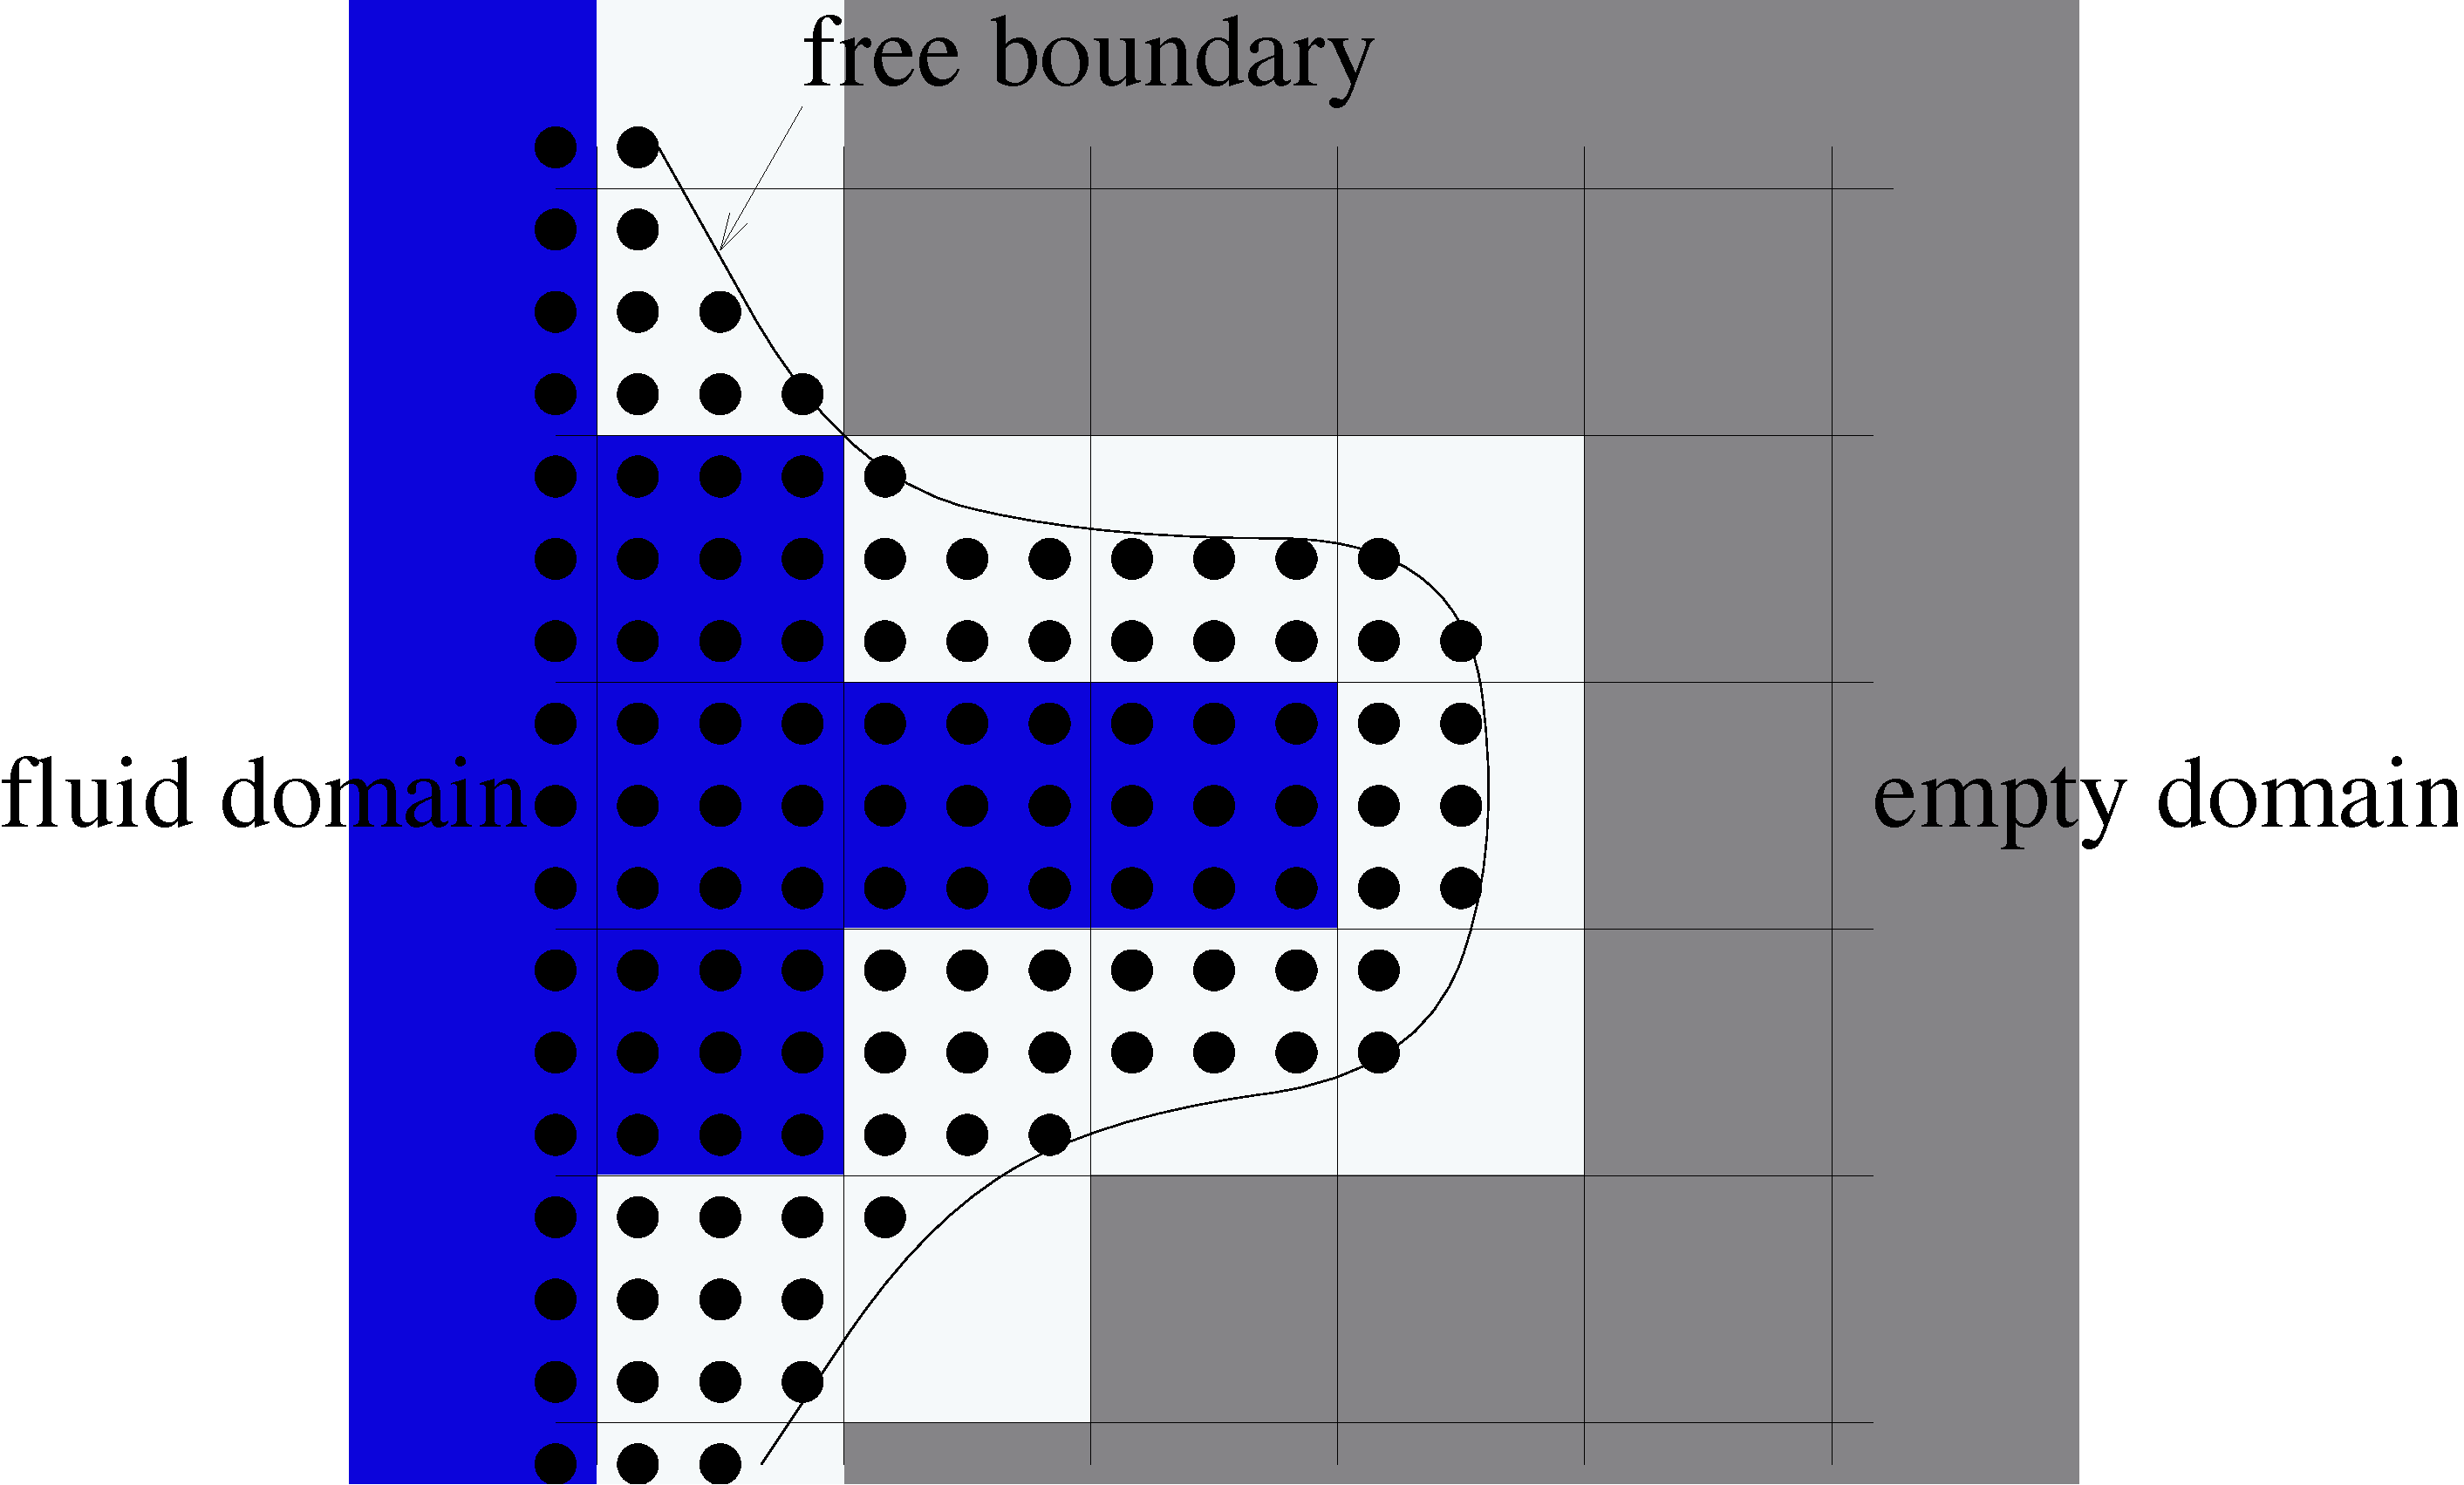
\includegraphics[height=0.8\textwidth]{pic/all.pdf}
			\end{figure}
		\end{column}
		\begin{column}[c]{0.6\textwidth}
			\begin{itemize}[<+->]
				\item the stress tensor:
					  $\ \sigma = (-P + \lambda div\vec{u})I+2 \mu \delta$					\item 
$\-P+\frac{2}{Re}(n_x n_x \frac{\partial u}{\partial x} + n_x n_y( \frac{\partial u}{\partial y} + \frac{\partial v}{\partial x} ) +  n_y n_y \frac{\partial v}{\partial y} ) = K \kappa  $					  						\item
 $2n_x m_x \frac{\partial u}{\partial x} +(n_x m_y + n_y m_x )( \frac{\partial u}{\partial y} + \frac{\partial v}{\partial x} ) + 2 n_y m_y \frac{\partial v}{\partial y} ) = 0 $
			\end{itemize}
		\end{column}
	\end{columns}
 \end{frame}	

\subsection{Free surface treatment}
	\begin{frame}{One empty neighbor}
	  \begin{columns}
	 	\begin{column}[c]{0.4\textwidth}
		 \begin{figure}
			\includegraphics[width=1\textwidth]{pic/one.pdf}
		 \end{figure}			
		\end{column}
			\begin{column}[c]{0.6\textwidth}
				\begin{itemize}
					\item  free boundary lie almost parallel to the grid lines
					\item $ n_y \& m_x=0	\~ OR   n_x \& m_y=0  $
					\item $ P=\frac{2}{Re} \frac{\partial u}{\partial x} $
					\item $ \frac{\partial u}{\partial y}+ \frac{\partial v}{\partial x}=0 $
					\item using continuity equation
				\end{itemize}
			\end{column}
	 \end{columns}
	\end{frame}	
	\begin{frame}{Two empty neighbor-common corner}
	    \begin{columns}
	 		\begin{column}[c]{0.4\textwidth}
		 		\begin{figure}
					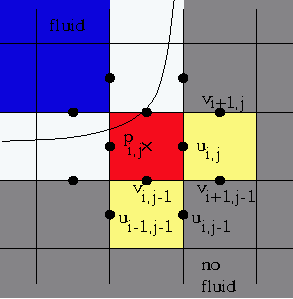
\includegraphics[width=1\textwidth]{pic/two1.pdf}
		 		\end{figure}
			\end{column}
			\begin{column}[c]{0.6\textwidth}
				\begin{itemize}
					\item $ n_y = m_x=n_x = m_y  $
					\item $ P=\pm \frac{1}{Re}( \frac{\partial u}{\partial x}+  \frac{\partial v}{\partial x} ) $
					\item $ \frac{\partial u}{\partial x}- \frac{\partial v}{\partial y}=0 $
				\end{itemize}
			\end{column}
		\end{columns}		
	\end{frame}	
	
	\begin{frame}{Two empty neighbor-opposite side}
	  \begin{columns}
	 	\begin{column}[c]{0.4\textwidth}
	 	\begin{figure}
			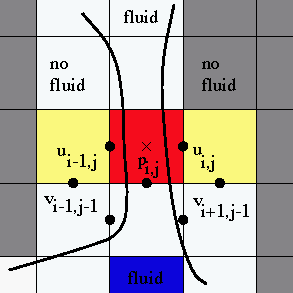
\includegraphics[width=0.49\textwidth]{pic/two2.pdf}
		 \end{figure}
		\end{column}
		\begin{column}[c]{0.6\textwidth}
				\begin{itemize}
					\item $ u_{i,j}^{new}= u_{i,j}^{old} +\delta t g_x $
					\item $ u_{i-1,j}^{new}= u_{i-1,j}^{old} +\delta t g_x $
					\item $ v_{i,j}^{new}= v_{i,j}^{old} +\delta t g_y $
					\item $ v_{i,j-1}^{new}= v_{i,j-1}^{old} +\delta t g_y $
				\end{itemize}
			\end{column}
		\end{columns}
	\end{frame}	
	
	\begin{frame}{Three empty neighbor}
	  \begin{columns}
	 	\begin{column}[c]{0.4\textwidth}
	 	   \begin{figure}
			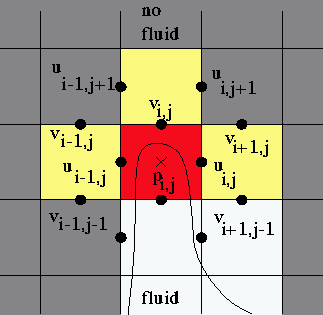
\includegraphics[width=0.49\textwidth]{pic/three.pdf}
			\end{figure}
		\end{column}
		\begin{column}[c]{0.4\textwidth}
	 	   \begin{figure}
	 	   			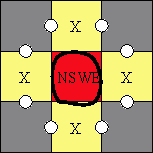
\includegraphics[width=0.49\textwidth]{pic/four.pdf}
			\end{figure}
		\end{column}
	\end{columns}
   \end{frame}	
		
 	
\section{Implementation} 
\subsection{Creating New Code}
\frame{\frametitle{Particle and ParticleTracer}
\begin{itemize}
\item \textbf{Particle(real x, real y, int type)} \\
Has some functions which can detect its position on the grid
\item \textbf{ParticleTracer(StaggeredGrid *grid)} \\
Has a vector of particles
\begin{itemize}
\item \textbf{void markCells()}
\item \textbf{void fillCell(int i, int j, int numParticles, int type)}
\item \textbf{void addRectangle(real x1, real y1, real x2, real y2, int type)}
\item \textbf{void addCircle(real x, real y, real r, int type)}
\item \textbf{void advanceParticles(real const dt)}
\end{itemize}
\end{itemize}
}

\subsection{Changing Old Classes And Functions}
\frame{\frametitle{Types and StaggeredGrid}
\begin{itemize}
\item \textbf{Types.hh}:
\begin{itemize}
\item \textbf{flag EMPTY}
\end{itemize}
\item \textbf{StaggeredGrid.cc}:
\begin{itemize}
\item \textbf{int ppc\_}
\item \textbf{bool isEmpty(const int x, const int y)}
\item \textbf{void setCellToEmpty(int x, int y)}
\item \textbf{void refreshEmpty()}
\end{itemize}
\end{itemize}
}
\frame{\frametitle{FluidSimulator}
\begin{itemize}
\item \textbf{FluidSimulator.cc}:
\begin{itemize}
\item \textbf{real rectX1\_particle\_, rectX2\_particle\_ , ...}
\item \textbf{real circR\_particle\_, circX\_particle\_, ...}
\item \textbf{void set\_UVP\_surface(int i, int j , const real \&dt, bool compP)}
\item \textbf{void one\_empty\_neighbour(int i , int j , const real \&dt, bool compP)}
\item ...
\item \textbf{four\_empty\_neighbour(int i , int j , const real \&dt, bool compP)}
\item \textbf{void refreshEmpty()}
\end{itemize}
\end{itemize}
}

\subsection{Main Algorithm}

\begin{frame}[fragile]
\frametitle{Main while-loop}
\lstset {language=C++}
\begin{lstlisting}
while (n <= nrOfTimeSteps)
{
    ...
    determineNextDT(safetyfac_);
    particle_tracer_.markCells();
    set_UVP_surface(dt_, true);
    computeFG();
    composeRHS();
    solv().solve(grid_);
    updateVelocities();
    refreshBoundaries();
    set_UVP_surface(dt_, false);
    particle_tracer_.advanceParticles(dt_);
    ...
}
\end{lstlisting}
\end{frame}

\section{Results}
\begin{frame}
\frametitle{Examples}
\begin{itemize}
\item The Breaking Dam - Outflow
\item The Breaking Dam - Freeslip
\item The Splash of a Liquid Drop
\end{itemize}
\end{frame}

\subsection{Parameters}
\begin{frame}[fragile]
\frametitle{The Breaking Dam}
\begin{lstlisting}
imax = 50,      jmax = 20,   
xlength = 10.0, ylength = 4.0,  
tau = 0.5,      delt = 0.04,   t_end = 5.0,
eps = 0.001,    omg = 1.7,   
gamma = 0.5,    itermax = 500,
GX = 0.0,       GY = -1.0,     Re = 10.0,
UI = 0.0,       VI = 0.0,      PI = 0.0,         
ppc=16,

wW = free,      wE=out,      
wS = free,      wN=out
\end{lstlisting}
\end{frame}

\begin{frame}[fragile]
\frametitle{The Splash of a Liquid Drop}
\begin{lstlisting}
imax = 40,      jmax = 30,   
xlength = 8.0,  ylength = 6.0,  
tau = 0.2,      delt = 0.01,   t_end = 10.0,
eps = 0.001,    omg = 1.7,   
gamma = 0.5,    itermax = 500,
GX = 0.0,       GY = -1.0,     Re = 40.0,
UI = 0.0,       VI = 0.0,      PI = 0.0,         
ppc=16,

wW = free,      wE=free,      
wS = free,      wN=out
\end{lstlisting}
\end{frame}

\end{document}
